\section{系统调用机制与中断}

中断是一种异步事件,它可以打断正在执行的程序并转移到处理中断的程序(中断处理程序)。
中断可以来自外部设备(如硬件中断)或软件(如系统调用)。中断机制是操作系统用来响应和处理中断的一种机制,
其中涉及中断向量表、中断控制器、中断处理程序等概念。

系统调用是中断的一种,通常情况下,U态的中断包括了系统调用,系统调用陷入内核态后,
将会调用SBI call来执行具体的内容。下面的\autoref{fig:syscall和SBI区别}清晰地展示了这两种中断的区别及联系。

\begin{figure}[htb]
    \centering
    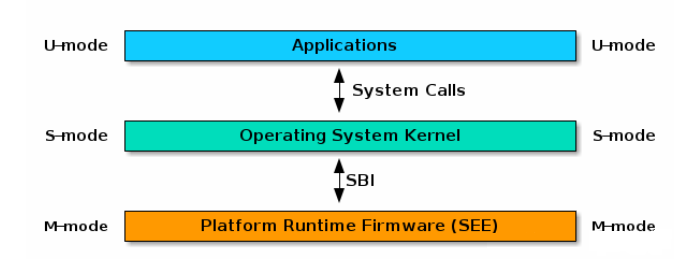
\includegraphics[width=\textwidth]{figures/03-03-syscall和SBI区别.png}
    \caption{
        syscall和SBI区别
    }
    \label{fig:syscall和SBI区别}
\end{figure}

系统调用是应用程序向操作系统请求服务的一种机制。应用程序无法直接访问操作系统内核的代码和数据结构,
因此需要通过系统调用来请求操作系统的服务。例如,在Linux操作系统中,应用程序可以通过系统调用请求创建新的进程、
读写文件、网络通信等操作。

同时,RISC-V使用SBI(Supervisor Binary Interface)作为系统调用的接口,提供了一组标准的系统调用函数,
包括控制台输出、内存分配、时钟等服务。

从系统调用以及中断的角度考虑,RISC-V使用TVEC(Trap Vector Base Address)寄存器来指定中断向量表的基地址,
中断向量表存储了中断处理程序的入口地址。当发生中断时,CPU会自动跳转到相应的中断处理程序,
并在处理完成后返回到中断前的指令位置。RISC-V还提供了一些相关的指令和寄存器,用于中断的使能、屏蔽和处理。

\autoref{fig:RISC-V的系统调用处理流程图}是riscv架构下对系统调用的处理流程。

\begin{figure}[htb]
    \centering
    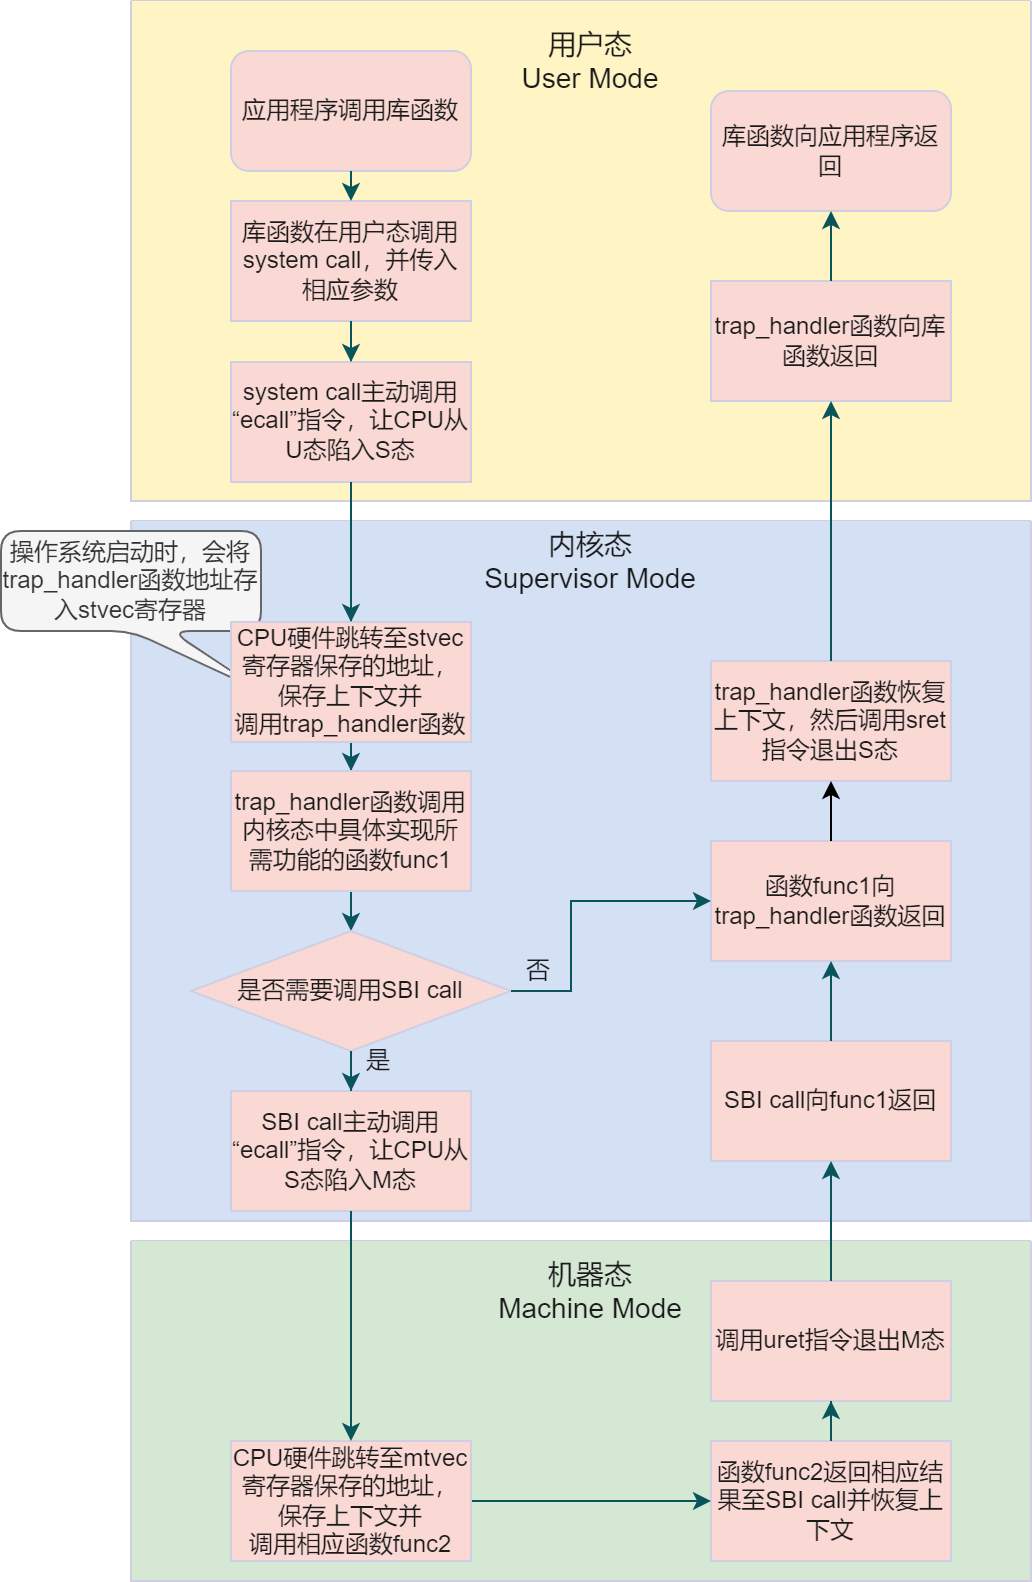
\includegraphics[width=0.5\textwidth]{figures/03-03-RISC-V的系统调用处理流程图.png}
    \caption{
        RISC-V的系统调用处理流程图
    }
    \label{fig:RISC-V的系统调用处理流程图}
\end{figure}

从本节开始,我们将正式开始学习NPUcore对于系统调用的真正处理和实现。
为了确保知识的合理递进,我们将其中最重要的内容分为了下面几个小节:

\begin{itemize}
    \item Trap及中断使能
    \item 系统调用与ecall指令
    \item 设置stvec寄存器及编写trap_handle函数
    \item 利用汇编实现上下文保存与恢复
    \item RustSBI简介及调用RustSBI
\end{itemize}

\subsection{Trap及中断使能}

\subsubsection{Trap的概念及其作用}

在上文中我们提到,系统调用是trap的一种,因此我们要了解系统调用,必须先了解trap是什么。

trap的3种类型:
\begin{enumerate}
    \item 主动的陷入:system call
    \item 外设中断处理:鼠标、键盘响应
    \item 运行时的意外:error、溢出、除0等
\end{enumerate}

每个RISC-V CPU都有一组控制寄存器,内核通过向这些寄存器写入内容来告诉CPU如何处理陷阱,
内核可以读取这些寄存器来明确已经发生的陷阱。RISC-V文档包含了完整的内容。riscv.h(kernel/riscv.h:1)
包含在NPUcore中使用到的内容的定义。\autoref{table:重要寄存器概述}是最重要的一些寄存器概述:

\begin{table}[h]
    \centering
    \caption{重要寄存器概述}
    \label{table:重要寄存器概述}
    \begin{tabularx}{0.8\textwidth}{|p{2cm}|X|}
    \hline
    \textbf{寄存器名称} & \textbf{功能}                                                     \\\hline
    stvec    & 内核在这里写入其陷阱处理程序的地址,RISC-V跳转到这里处理陷阱                     \\\hline
    sepc     & 当发生陷阱时,RISC-V会在这里保存程序计数器pc(因为pc会被stvec覆盖)              \\\hline
    sret     & (从陷阱返回)指令会将sepc复制到pc,内核可以写入sepc来控制sret的去向              \\\hline
    scause   & RISC-V在这里放置一个描述陷阱原因的数字                                         \\\hline
    sscratch & 内核在这里放置了一个值,这个值在陷阱处理程序一开始就会派上用场                    \\\hline
    sstatus  & 其中的SIE位控制设备中断是否启用。如果内核清空SIE,RISC-V将推迟设备中断,          
               直到内核重新设置SIE。SPP位指示陷阱是来自用户模式还是管理模式,并控制sret返回的模式 \\\hline
    \end{tabularx}
\end{table}

\subsubsection{使能中断}

使能中断指的是在CPU中打开中断处理的能力。如果中断被禁用,即使有中断请求发生,CPU也不会执行中断处理程序,
而是继续执行当前的任务,直到中断被启用为止。一旦中断被启用,当有中断请求发生时,
CPU会在适当的时候挂起当前的任务,跳转到中断处理程序,执行完毕后再返回到原来的任务。

在RISC-V架构中,使能中断可以通过设置sstatus寄存器下的SIE位来打开或关闭的中断使能。
当相应的寄存器被置为1时,对应的中断将被使能。

\begin{figure}[htb]
    \centering
    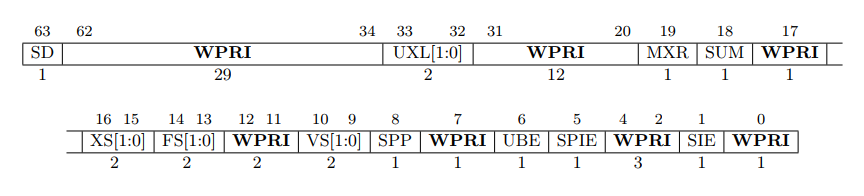
\includegraphics[width=\textwidth]{figures/03-03-SXLEN=64时S-mode下的状态寄存器(sstatus).png}
    \caption{
        SXLEN=64时S-mode下的状态寄存器(sstatus)
    }
    \label{fig:SXLEN=64时S-mode下的状态寄存器(sstatus)}
\end{figure}

在NPUcore中,为了确保中断与系统调用可用,我们利用RustSBI进行了如下的操作:

\begin{lstlisting}[language={Rust}]
unsafe {
    riscv::register::sstatus::set_sie();
}
\end{lstlisting}

该操作实际上是对sstatus寄存器的低1位赋值为1,这样便打开了中断使能。

\subsection{系统调用与ecall指令}

在RISC-V架构下,系统调用是通过ecall指令来触发的。ecall指令是一条特殊的指令,当我们在U态执行ecall指令时,
会跳转到STVEC寄存器中函数地址指定的中断处理程序,即系统调用处理程序
(若是在S态触发ecall,则会跳转到mtvec存储的函数地址),进行相应的操作。
ecall指令一般用来触发一些特殊的操作,比如系统调用、中断、异常等。

当我们在U态利用系统调用出发ecall指令后,需要进行相应的操作,比如将参数传递到内核态,由内核态进行相应的操作,
然后再将结果返回给用户态。在系统调用发生时,需要将当前用户态的上下文保存起来,这样在系统调用完成后,
CPU就可以从保存的上下文中恢复用户态的执行状态。

接下来,我们通过NPUcore具体的代码实例来学习如何利用ecall指令来完成系统调用。

我们以write系统调用为例,来详细描述系统调用的具体流程。

\subsubsection{用户态进程调用syscall}

\begin{itemize}
    \item 应用程序调用位于user/src/usr_call.rs中被包装好的write函数;
    \item write函数调用位于user/src/usr_call.rs中的sys_write函数;
\end{itemize}

应用程序如何想使用操作系统为其提供的服务,最直接的办法就是调用操作系统提供的库函数。

NPUcore的设计正是如此,我们将syswrite函数进行了一次包装,放在user/src/usr_call.rs中,模拟库函数,
见\autoref{code:usr call write}。

我们对sys_write传递两个参数,分别是文件描述符fd以及缓冲区指针buf。

\begin{lstlisting}[language={Rust}, label={code:usr call write},
    caption={usr_call.rs:write}]
pub fn write(fd: usize, buf: &[u8]) -> isize {
    sys_write(fd, buf)
}
\end{lstlisting}

\begin{itemize}
    \item sys_write函数调用位于user/src/usr_call.rs中的syscall函数;
\end{itemize}

见\autoref{code:usr call sys write},我们的包装类似于lib库函数,利用sys_write函数来调用syscall。

\begin{lstlisting}[language={Rust}, label={code:usr call sys write},
    caption={usr_call.rs:sys_write}]
pub fn sys_write(fd: usize, buffer: &[u8]) -> isize {
    syscall(SYSCALL_WRITE, [fd, buffer.as_ptr() as usize, buffer.len()])
}
\end{lstlisting}

\subsubsection{syscall调用ecall指令陷入内核态}

syscall函数中内联的汇编函数执行了ecall,陷入内核态。每一个syscall都有4个参数,
第一个参数代表着系统调用的id,NPUcore的系统调用标识完全遵循linux标准,因此可以方便地兼容linux操作系统的应用程序。
其余三个参数供每个系统调用进行灵活选择。

\begin{lstlisting}[language={Rust}, label={code:syscall},
    caption={syscall}]
fn syscall(id: usize, args: [usize; 3]) -> isize {
    let mut ret: isize;
    unsafe {
        asm!(
            "ecall",
            inlateout("x10") args[0] => ret,
            in("x11") args[1],//分别把参数放进a1、a2、a7
            in("x12") args[2],
            in("x17") id
        );
    }
    ret
}
\end{lstlisting}

见\autoref{code:syscall},在第五行,第一条指令就是ecall指令,我们在此调用ecall指令触发trap,使得程序陷入内核态
第六行的inlateout指令有两个作用:一是把args[0]放进a0寄存器;二是在程序返回后x10寄存器会作为返回值。
接下来三行就是参数的传递。

至此,我们已经完成了系统调用在用户空间中应该进行的操作。

\subsection{设置stvec寄存器与编写trap_handle函数}

在用户态进程调用ecall进入内核态后,CPU将会自动进行如下操作:

\begin{itemize}
    \item sstatus 的 SPP 字段会被修改为 CPU 当前的特权级(U/S)。
    \item sepc 会被修改为 Trap 处理完成后默认会执行的下一条指令的地址。
    \item scause/stval 分别会被修改成这次 Trap 的原因以及相关的附加信息。
    \item CPU 会跳转到 stvec 所设置的 Trap 处理入口地址,并将当前特权级设置为 S ,然后从Trap 处理入口地址处开始执行。
\end{itemize}

在这些操作中,我们最需要关心的是第四点。

尽管上文已经提到了stvec寄存器的具体功能,但仍然在这强调一下该寄存器的具体作用:
在RISC-V架构中,中断控制器寄存器写入的是中断向量表的基地址(Base Address)。
stvec寄存器用于存储中断向量表的基地址,并指定了中断向量表的模式(Direct Mode或Vectored Mode)。
当中断处理器接收到一个中断信号时,会根据stvec寄存器的值,自动跳转到中断向量表中对应的中断处理程序的入口地址。

因为硬件实现了自动跳转到stvec寄存器的功能,因此接下来我们只需要考虑如何往stvec寄存器中写入内容,以及写入什么内容。
这两个问题的回答正是我们这一小节的主题——设置stvec寄存器及编写trap_handle函数。

\subsubsection{设置stvec寄存器}

我们应该向stvec写入什么呢?答案是显而易见的——中断处理函数。

其实,在操作系统初始化的时候,就已经修改了 stvec 寄存器来指向正确的 Trap 处理入口点,
见\autoref{code:set user trap entry}。

\begin{lstlisting}[language={Rust}, label={code:set user trap entry},
    caption={set_user_trap_entry}]
fn set_user_trap_entry() {
    unsafe {
        stvec::write(TRAMPOLINE as usize, TrapMode::Direct);
    }
}
\end{lstlisting}

这里引入了一个外部符号 TRAMPOLINE(意为跳板) ,并将 stvec 设置为 Direct 模式指向它的地址。
在 os/src/trap/trap.S 中实现 Trap 上下文保存/恢复的汇编代码,分别用外部符号 __alltraps 和 __restore 标记为函数,
并通过 global_asm! 宏将 trap.S 这段汇编代码插入进来。

为什么我们不直接将__alltraps符号写入stvec寄存器,而是要建立一个跳板?
使用跳板是为了解决这样一个问题:
在开启分页模式之后__alltraps的实际程序入口并不是一个特定值,而是取决于所处平台的不同(qemu/k210/u740)
以及在编译器/汇编器/链接器进行后端代码生成和链接形成最终机器码时设置好的此指令的地址。

从上文中我们可以知道,在编写 trap.S 中的整段汇编代码时,我们将这段代码放置在 .text.trampoline 段。

该符号在os/src/linker-k210.ld、os/src/linker-fu740.ld及os/src/qemu.ld被连接,
并在调整内存布局的时候将它对齐到代码段的一个页面中,见\autoref{code:linker-xxx-.ld}。

\begin{lstlisting}[label={code:linker-xxx-.ld},
    caption={linker-xxx-.ld}]
stext = .;
.text : {
    *(.text.entry)
    . = ALIGN(4K);
    strampoline = .;
    *(.text.trampoline);
    . = ALIGN(4K);
    ssignaltrampoline = .;
    KEEP(*(.text.signaltrampoline));
    . = ALIGN(4K);
    *(.text .text.*)
}
\end{lstlisting}

这样,这段汇编代码放在一个物理页帧中,且 __alltraps 恰好位于这个物理页帧的开头,
其物理地址被外部符号 strampoline 标记。在开启分页模式之后,内核和应用代码都只能看到各自的虚拟地址空间,
而在它们的视角中,这段汇编代码都被放在它们各自地址空间的最高虚拟页面上,
由于这段汇编代码在执行的时候涉及到地址空间切换,故而被称为跳板页面。

这样就可以解释为何在 __alltraps 中需要借助寄存器 jr 而不能直接 call trap_handler 了。
因为在内存布局中,这条 .text.trampoline 段中的跳转指令和 trap_handler 都在代码段之内,
汇编器(Assembler)和链接器(Linker)会根据 linker-qemu/k210.ld 的地址布局描述,设定跳转指令的地址,
并计算二者地址偏移量,让跳转指令的实际效果为当前 pc 自增这个偏移量。
但实际上由于我们设计的缘故,这条跳转指令在被执行的时候,它的虚拟地址被操作系统内核设置在地址空间中的最高页面之内,
所以加上这个偏移量并不能正确的得到 trap_handler 的入口地址。

在完成了这一步骤后,接下来将正式开始在S态中的中断处理流程。

\subsubsection{编写trap_handler函数}

在完成上文所述的设置stvec寄存器跳转地址后,我们将完成后续步骤:

\begin{enumerate}
    \item 通过 __alltraps 将 Trap 上下文保存在内核栈上。
    \item 跳转到使用 Rust 编写的 trap_handler 函数完成 Trap 分发及处理。
    \item 当 trap_handler 返回之后,使用 __restore 从保存在内核栈上的 Trap 上下文恢复寄存器。
    \item 最后通过一条 sret 指令回到应用程序执行。
\end{enumerate}

本节重点讲解其中的第二点,追踪NPUcore中trap_handler函数的具体实现流程并了解其核心思想。
由于该函数过长,这里只选取其中有关系统调用的部分进行讲解,见\autoref{code:trap handler}。

\begin{lstlisting}[language={Rust}, label={code:trap handler},
    caption={trap_handler}]
pub fn trap_handler() -> ! {
    set_kernel_trap_entry();
	//...
    let scause = scause::read();
    match scause.cause() {
        Trap::Exception(Exception::UserEnvCall) => {
            let mut cx = current_trap_cx();
            cx.gp.pc += 4;
            let result = syscall(
                cx.gp.a7,
                [cx.gp.a0, cx.gp.a1, cx.gp.a2, cx.gp.a3, cx.gp.a4, cx.gp.a5],
            );
            cx = current_trap_cx();
            cx.gp.a0 = result as usize;
        }
	//...
    trap_return();
}
\end{lstlisting}

在函数的开始,代码第2行,调用了set_kernel_trap_entry函数,在内核态的陷入是什么情况呢?
报错!这个函数定义了如果在内核态再发生Trap,会直接panic报错,是为了防止不正常的S->S态Trap的发生。

在第5行的match匹配,这个处理系统调用的子块函数做了三件事:
第一步,让pc+4,是为了跳转后能正确执行下一条指令。
第二步,把scause寄存器的值取出,调用os/src/syscall/mod.rs里面的syscall函数。
第三步,将返回值存入返回值寄存器a0中。

为什么在用户空间中有一个syscall函数,在内核空间中又会出现一个同名的syscall函数呢?
其实只有用户空间那个syscall才是我们平常意义上所说的系统调用,因为只有该syscall才调用了ecall指令,完成了trap操作。
而在内核空间中出现的syscall可以认为是对系统调用所需要完成的不同功能进行分发处理。

内核空间中出现的syscall在os/src/syscall/mod.rs中。
由于该函数过长,只选取其中少数几个的match项,见\autoref{code:syscall}。
示例该函数只是起一个根据系统调用号对操作进行分发的作用。

\begin{lstlisting}[language={Rust}, label={code:syscall},
    caption={syscall}]
pub fn syscall(syscall_id: usize, args: [usize; 6]) -> isize {
	//log
    let ret = match syscall_id {
        SYSCALL_GETCWD => sys_getcwd(args[0], args[1]),
        SYSCALL_DUP => sys_dup(args[0]),
        SYSCALL_DUP3 => sys_dup3(args[0], args[1], args[2] as u32),
        SYSCALL_FCNTL => sys_fcntl(args[0], args[1] as u32, args[2]),
        SYSCALL_IOCTL => sys_ioctl(args[0], args[1] as u32, args[2]),
       //...still more
    };
    ret
}
\end{lstlisting}

最后,在 trap_handler 完成 Trap 处理之后,调用 trap_return 返回用户态,见\autoref{code:trap return}。

\begin{lstlisting}[language={Rust}, label={code:trap return},
    caption={trap_return}]
fn set_user_trap_entry() {
    unsafe {
        stvec::write(TRAMPOLINE as usize, TrapMode::Direct);
    }
}

#[no_mangle]
pub fn trap_return() -> ! {
    set_user_trap_entry();
    let trap_cx_ptr = TRAP_CONTEXT;
    let user_satp = current_user_token();
    extern "C" {
        fn __alltraps();
        fn __restore();
    }
    let restore_va = __restore as usize - __alltraps as usize + TRAMPOLINE;
    unsafe {
        asm!(
            "fence.i",
            "jr {restore_va}",
            restore_va = in(reg) restore_va,
            in("a0") trap_cx_ptr,
            in("a1") user_satp,
            options(noreturn)
        );
    }
    panic!("Unreachable in back_to_user!");
}
\end{lstlisting}

\begin{itemize}
    \item 第 11 行,在 trap_return 的开始处调用 set_user_trap_entry ,
    来让应用 Trap 到 S 的时候可以跳转到 __alltraps 。
    注意,需要把 stvec 设置为内核和应用地址空间共享的跳板页面的起始地址 TRAMPOLINE ,
    而不是编译器在链接时看到的 __alltraps 的地址。
    这是因为启用分页模式之后,内核只能通过跳板页面上的虚拟地址来实际取得 __alltraps 和 __restore 的汇编代码。

    \item 第 18 行,展示了计算 __restore 虚地址的过程:
    由于 __alltraps 是对齐到地址空间跳板页面的起始地址 TRAMPOLINE 上的, 
    则 __restore 的虚拟地址只需在 TRAMPOLINE 基础上加上 __restore 相对于 __alltraps 的偏移量即可。
    这里 __alltraps 和 __restore 都是指编译器在链接时看到的内核内存布局中的地址。

    \item 第 20-27 行,首先需要使用 fence.i 指令清空指令缓存 i-cache 。
    因为在内核中进行的一些操作,可能导致一些原先存放某个应用代码的物理页帧,如今用来存放数据或者是其他应用的代码。
    i-cache 中可能还保存着该物理页帧的错误快照。因此我们直接将整个 i-cache 清空避免错误。
    接着使用 jr 指令完成了跳转到 __restore 的任务。
\end{itemize}

\subsection{利用汇编实现上下文保存与恢复}

再回顾一下操作系统在S态对于系统调用的处理会经历的步骤:

\begin{enumerate}
    \item 通过 __alltraps 将 Trap 上下文保存在内核栈上。
    \item 跳转到使用 Rust 编写的 trap_handler 函数完成 Trap 分发及处理。
    \item 当 trap_handler 返回之后,使用 __restore 从保存在内核栈上的 Trap 上下文恢复寄存器。
    \item 最后通过一条 sret 指令回到应用程序执行。
\end{enumerate}

上一小节介绍了第二步,这一小节来介绍剩余三步,均是通过汇编代码来实现的,故先介绍一下RISC-V汇编的基础知识。

\subsubsection{RISC-V汇编基础知识}

首先看一下RISC-V汇编常用指令,见\autoref{tab:RISC-V汇编常用指令}。
其中CSR寄存器,即Control and Status Register,控制与状态寄存器。

\begin{table}[h]
    \centering
    \caption{RISC-V汇编常用指令}
    \label{table:RISC-V汇编常用指令}
    \begin{tabularx}{0.8\textwidth}{|p{1cm}|p{3cm}|X|}
    \hline
    \textbf{名称} & \textbf{格式} & \textbf{功能}                                      \\\hline
    sd     & sd rs2, offset(rs1) & 把寄存器rs2的值存入地址为寄存器rs1的值加offset的主存中 \\\hline
    ld     & ld rd, offset(rs1)  & 从地址为寄存器rs1的值加offset的主存中读取并存入rd      \\\hline
    csrr   & csrr rd, csr        & 读取CSR寄存器的值                                    \\\hline
    csrw   & csrw csr, rs        & 写入CSR寄存器                                       \\\hline
    csrrw  & csrrw rd, csr, rs1  & 读取CSR的旧值,写入rd寄存器,同时将rs1的值写入CSR     \\\hline
    jr     & jr rs               & 跳转到rs寄存器中的地址,并且不带返回值                \\\hline
    \end{tabularx}
\end{table}

为了更好的调用汇编指令,宏操作是一个很有效的手段。
.MACRO和.ENDM伪指令可以用来组成一个宏。.MACRO伪指令的格式如下

\begin{lstlisting}[]
.macro macname macargs ...
\end{lstlisting}

.MACRO伪指令后面依次是宏名称与宏的参数。
在宏里使用参数,需要添加前缀\lstinline`\`。

在正式编写函数前,声明了四个宏,作用分别是:
保存整数寄存器,恢复整数寄存器,保存浮点寄存器,恢复浮点寄存器。
见\autoref{code:riscv macro}。

\begin{lstlisting}[language={riscv}, label={code:riscv macro},
    caption={RISC-V宏}]
.altmacro
.macro SAVE_GP n
    sd x\n, \n*8(sp)
.endm
.macro LOAD_GP n
    ld x\n, \n*8(sp)
.endm
.macro SAVE_FP n, m
    fsd f\n, \m*8(sp)
.endm
.macro LOAD_FP n, m
    fld f\n, \m*8(sp)
.endm
\end{lstlisting}

有了上述RISC-V汇编的基础知识,接下来正式开始讲解__alltraps与__restore。

\subsubsection{保存上下文:__alltraps}

\begin{lstlisting}[language={riscv}, label={code:alltraps},
    caption={__alltraps}]
__alltraps:
    csrrw sp, sscratch, sp
    # now sp->*TrapContext in user space, sscratch->user stack
    sd x1, 1*8(sp)
    # skip sp(x2), we will save it later
    .set n, 3
    .rept 29
        SAVE_GP %n
        .set n, n+1
    .endr
    .set n, 0
    .set m, FP_START
    .rept 32
        SAVE_FP %n, %m
        .set n, n+1
        .set m, m+1
    .endr
    # we can use t0/t1/t2 freely, because they have been saved in TrapContext
    csrr t0, fcsr
    sd t0, 64*8(sp)
    # save other general purpose registers
    sd a0, 65*8(sp)
    csrr t0, sstatus
    csrr t1, sepc
    sd t0, 66*8(sp)
    sd t1, 0(sp)
    # read user stack from sscratch and save it in TrapContext
    csrr t2, sscratch
    sd t2, 2*8(sp)
    # load kernel_satp into t0
    ld t0, 67*8(sp)
    # load trap_handler into t1
    ld t1, 68*8(sp)
    # move to kernel_sp
    ld sp, 69*8(sp)
    # switch to kernel space
    csrw satp, t0
    sfence.vma
    # jump to trap_handler
    jr t1
\end{lstlisting}

第 2 行的 csrrw 原型是 \lstinline`csrrw rd, csr, rs`' 可以将 CSR 当前的值读到通用寄存器 rd 中,
然后将通用寄存器 rs 的值写入该 CSR 。因此这里起到的是交换 sscratch 和 sp 的效果。
在这一行之前 sp 指向用户栈, sscratch 指向内核栈,现在 sp 指向内核栈, sscratch 指向用户栈。

第 4 行,保存 Trap 上下文的通用寄存器 x1。

在这里不保存 sp(x2),因为要基于它来找到每个寄存器应该被保存到的正确的位置。
实际上,在栈帧分配之后,我们可用于保存 Trap 上下文的地址区间为 [sp,sp+8×34) ,
按照 TrapContext 结构体的内存布局,基于内核栈的位置(sp所指地址)
来从低地址到高地址分别按顺序放置 x0-x31这些通用寄存器,最后是 sstatus 和 sepc 。

第 6-10 行,为了简化代码,x3~x31 这 29 个通用寄存器通过类似循环的 .rept 每次使用 SAVE_GP 宏来保存,
其实质是相同的。注意我们需要在 trap.S 开头加上 .altmacro 才能正常使用 .rept 命令。

第 11-17 行,用类似的方法,保存浮点寄存器。

第 23-26行,将 CSR sstatus 和 sepc 的值分别读到寄存器 t0 和 t1 中然后保存到内核栈对应的位置上。
指令 csrr rd, csr 的功能就是将 CSR 的值读到寄存器 rd 中。这里不用担心 t0 和 t1 被覆盖,
因为它们刚刚已经被保存了。

第 28-29 行专门处理 sp 的问题。首先将 sscratch 的值读到寄存器 t2 并保存到内核栈上,
注意: sscratch 的值是进入 Trap 之前的 sp 的值,指向用户栈。而现在的 sp 则指向内核栈。

31-40行,切换到内核地址空间并跳转到 trap handler 。

\begin{itemize}
    \item 第 31 行将内核地址空间的 token 载入到 t0 寄存器中;
    \item 第 33 行将 trap handler 入口点的虚拟地址载入到 t1 寄存器中;
    \item 第 35 行直接将 sp 修改为应用内核栈顶的地址;\\
    注:这三条信息均是内核在初始化该应用的时候就已经设置好的。
    \item 第 37~38 行将 satp 修改为内核地址空间的 token 并使用 sfence.vma 刷新快表,这就切换到了内核地址空间;
    \item 第 40 行 最后通过 jr 指令跳转到 t1 寄存器所保存的trap handler 入口点的地址。
\end{itemize}

\subsubsection{恢复上下文:__restore}

\begin{lstlisting}[language={riscv}, label={code:restore},
    caption={__restore}]
__restore:
    # a0: *TrapContext in user space(Constant); a1: user space token
    # switch to user space
    csrw satp, a1
    sfence.vma
    csrw sscratch, a0
    mv sp, a0
    # now sp points to TrapContext in user space, start restoring based on it
    # restore sstatus/sepc
    ld t0, 32*8(sp)
    ld t1, 33*8(sp)
    csrw sstatus, t0
    csrw sepc, t1
    # restore general purpose registers except x0/sp/tp
    ld x1, 1*8(sp)
    ld x3, 3*8(sp)
    .set n, 5
    .rept 27
        LOAD_GP %n
        .set n, n+1
    .endr
    # back to user stack
    ld sp, 2*8(sp)
    sret
\end{lstlisting}

当内核将 Trap 处理完毕准备返回用户态的时候会 调用 __restore ,它有两个参数:
第一个是 Trap 上下文在应用地址空间中的位置,这个对于所有的应用来说都是相同的,
在 a0 寄存器中传递;第二个则是即将回到的应用的地址空间的 token ,在 a1 寄存器中传递。

第 4~5 行先切换回应用地址空间(注:Trap 上下文是保存在应用地址空间中);

第 6 行将传入的 Trap 上下文位置保存在 sscratch 寄存器中,
这样 __alltraps 中才能基于它将 Trap 上下文保存到正确的位置;

第 7 行将 sp 修改为 Trap 上下文的位置,后面基于它恢复各通用寄存器和 CSR;

第 24 行最后通过 sret 指令返回用户态。完成了一次完整的系统调用。


\subsection{RustSBI简介与调用RustSBI}

\subsubsection{RustSBI简介}

经过系统调用陷入S态后,如果S态的内核程序无法独立地完成U态应用程序所需的功能,
则它必须要再调用SBI call,以请求M态程序SBI的服务。

RISC-V指令集的SBI标准规定了类Unix操作系统之下的运行环境规范。这个规范拥有多种实现,RustSBI是它的一种实现。

RISC-V架构中,存在着定义于操作系统之下的运行环境。这个运行环境不仅将引导启动RISC-V下的操作系统, 
还将常驻后台,为操作系统提供一系列二进制接口,以便其获取和操作硬件信息。 
RISC-V给出了此类环境和二进制接口的规范,称为“操作系统二进制接口”,即“SBI”。
SBI的实现是在M模式下运行的特定于平台的固件,它将管理S、U等特权上的程序或通用的操作系统。

RustSBI是RISC-V下SBI标准的实现,旨在为裸机平台、虚拟化和模拟器软件提供良好的SBI接口支持。
它有机结合了Rust嵌入式生态与RISC-V系统软件,加快开发速度的同时,保证Rust语言具备的良好安全性和运行性能。
本次0.3.0版本主要包括增加了实例化的SBI接口支持及相关的构造器结构,可以在stable Rust编译,去
除了对堆内存和全局变量的依赖,完善了相关文档,以及若干的小修复。
0.3.0版本更新将为Rust编写的RISC-V虚拟化软件和RISC-V模拟器提供良好的支持,
并进一步完善裸机RISC-V开发的实用性,可以启动Linux等在内的成熟操作系统和zCore等在内的科研操作系统。

若想了解更多有关RustSBI的知识和具体实现,请前往开发者洛佳的github仓库:
https://github.com/rustsbi/rustsbi

\subsubsection{在NPUcore中调用RustSBI}

与我们在U态使用ecall指令调用syscall并陷入内核态那样,
我们在内核态同样也可以通过ecall指令调用RustSBI并进一步陷入M态。

正如我们会给syscall进行系统调用编号那样,我们也可以通过寄存器传递给OpenSBI一个“调用编号”。

SBI的规范中为SBI call定义了9个编号,见\autoref{code:sbi call numbers}

\begin{lstlisting}[language={Rust}, label={code:sbi call numbers},
    caption={SBI call 调用编号}]
const SBI_SET_TIMER: usize = 0;
const SBI_CONSOLE_PUTCHAR: usize = 1;
const SBI_CONSOLE_GETCHAR: usize = 2;
const SBI_CLEAR_IPI: usize = 3;
const SBI_SEND_IPI: usize = 4;
const SBI_REMOTE_FENCE_I: usize = 5;
const SBI_REMOTE_SFENCE_VMA: usize = 6;
const SBI_REMOTE_SFENCE_VMA_ASID: usize = 7;
const SBI_SHUTDOWN: usize = 8;
\end{lstlisting}

在S态调用SBI call的方法与U态调用syscall的方法类似,通过\autoref{code:syscall sbi call}来具体观察。

\begin{lstlisting}[language={Rust}, label={code:syscall sbi call},
    caption={syscall与SBI call对比}]
fn syscall(id: usize, args: [usize; 3]) -> isize {
    let mut ret: isize;
    unsafe {
        asm!(
            "ecall",
            inlateout("x10") args[0] => ret,
            in("x11") args[1],
            in("x12") args[2],
            in("x17") id
        );
    }
    ret
}
fn sbi_call(which: usize, arg0: usize, arg1: usize, arg2: usize) -> usize {
    let mut ret;
    unsafe {
        asm!(
            "ecall",
            inlateout("x10") arg0 => ret,
            in("x11") arg1,
            in("x12") arg2,
            in("x17") which,
        );
    }
    ret
}
\end{lstlisting}

可以发现二者几乎相同。这个现象引出来一个问题:既然我们在U态进行系统调用时,
保存与恢复用户态寄存器上下文的内容是由内核程序完成的(见上述章节),
那么我们现在在内核态进行SBI call,保存与恢复内核态寄存器的上下文是不是应该由SBI程序完成呢?

查看SBI的实现规范文档得知,以上猜测是正确的。此外,
与内核程序中需要设置stvec寄存器以正确跳转至trap_handler函数一样,RustSBI也同样设置了mtvec寄存器。

因此,在编写系统调用乃至整个NPUcore的过程中,由于RustSBI的存在,机器级硬件的操控基本被屏蔽了,
可以把心思专心放在内核态程序的编写中来。